\section{Представление алгоритмов. Блок-схемы}

\textbf{Алгоритм} -- это точное предписание, определяющее вычислительный
процесс, ведущий от варьируемых начальных данных к искомому результату.

Алгоритм может быть представлен различным образом:
\begin{enumerate}
\item
  Словесный;

  Предполагает описание алгоритма на естественном языке. Имеет существенный недостаток - строго не формализуем.

\item
  Формульно-словесный;

  Алгоритм записывается в виде текста с формулами по пунктам,
  определяющим последовательность действий.
\item
  \textbf{Блок-схемный};
\item
  Псевдокод;

  \emph{Псевдокод} - компактный, зачастую неформальный язык описания
  алгоритмов, использующий ключевые слова императивных языков
  программирования, но опускающий несущественные для понимания алгоритма
  подробности и специфический синтаксис.
\item
  Структурные диаграммы;

  \emph{Структурные диаграммы} описывают структуру сложных объектов и
  систем, показывают статическую структуру системы и ее частей на разных
  уровнях абстракции и реализации, а также их взаимосвязь.
\item
  Языки программирования

  \emph{Алгоритмический язык} --- это искусственный язык (система
  обозначений), предназначенный для записи алгоритмов. Он позволяет
  представить алгоритм в виде текста, составленного по определенным
  правилам с использованием специальных служебных слов. Количество таких
  слов ограничено. Каждое служебное слово имеет точно определенный
  смысл, назначение и способ применения.

  \textbf{Язык программирования} - алгоритмический язык, команды
  которого однозначно преобразуются в команды для компьютера.
\end{enumerate}

\subsection{Блок-схемы}\label{ux431ux43bux43eux43a-ux441ux445ux435ux43cux44b}

\textbf{Блок--схема} --- наглядный способ представления алгоритма.
Блок--схема отображается в виде последовательности связанных между собой
\emph{функциональных блоков}, каждый из которых соответствует выполнению
одного или нескольких действий. Определенному типу действия
соответствует \emph{определенная геометрическая фигура блока} (см. рисунок \ref{fig:schematic}). Линии,
соединяющие блоки, определяют \emph{очередность выполнения действий}. По
умолчанию блоки соединяются \emph{сверху вниз и слева направо}. Если
последовательность выполнения блоков должна быть иной, используются
направленные линии (стрелки).

\begin{figure}[h]
\centering
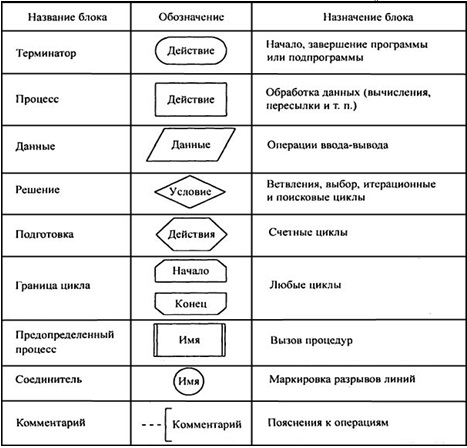
\includegraphics[width=0.5\textwidth]{./res/schematics.png}
\caption{Обозначения на блок-схемах}
\label{fig:schematic}
\end{figure}

Блок-схемы регламентируются такими документами, как \textbf{ГОСТ
19.701-90}, \textbf{СТП 01-2017} (стандарт предприятия БГУИР).

Пример блок-схемы алгоритма (рисунок -1).
